\section{実験目的}

先行研究\cite{mura}と同様の実験を行い様々な雨量の雨天環境の2D LiDARデータを取得することを目的とする.

\section{実験装置}

実験装置は先行研究\cite{mura}と同様である.
実験装置として本研究室で開発しているロボットORNE-box2\cite{orne}を使用する.
ロボットの外観と仕様を\figref{Fig:4.1}と\tabref{table:ORNE-box2}に示す.
また,使用した2D LiDAR(UTM-30LX-EW)の外観と仕様を\figref{Fig:4.2}と\tabref{table:angular}に示す.

\begin{figure}[H]
  \centering
  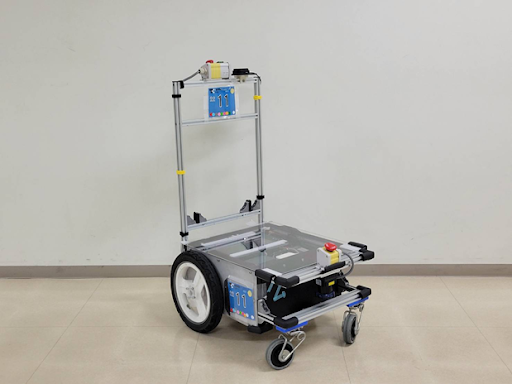
\includegraphics[keepaspectratio, scale=0.4]{images/png/orne-box2.png}
  \caption{ORNE-box2(source:\cite{mura})}
  \label{Fig:4.1}
\end{figure}

\newpage
\vspace{10zh}

\begin{table}[H]
  \centering
  \caption[Specifications of ORNE-box2]{Specifications of ORNE-box2(source:\cite{mura}\cite{orne})}
  \begin{tabular}{|l|l|}
  \hline
  Depth {[}mm{]}          & 600 \\ \hline
  Width {[}mm{]}          & 507 \\ \hline
  Height {[}mm{]}         & 957 \\ \hline
  Wheel diameter {[}mm{]} & 304 \\ \hline
  Weight {[}kg{]}         & 30  \\ \hline
  \end{tabular}
  \label{table:ORNE-box2}
  \end{table}

\vspace{10zh}
\begin{figure}[H]
  \centering
  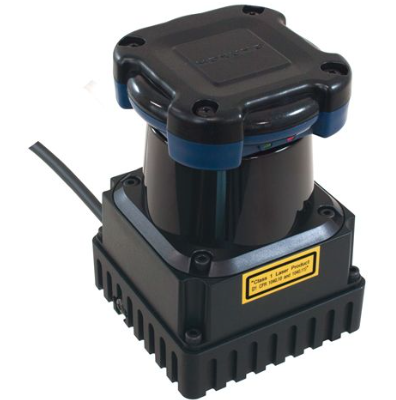
\includegraphics[keepaspectratio, scale=0.6]{images/png/LiDAR.png}
  \caption{2D LiDAR(UTM-30LX-EW)(source:\cite{lidar})}
  \label{Fig:4.2}
\end{figure}


  \begin{table}[H]
    \small
    \centering
    \caption[Specifications of Hokuyo UTM-30LX-EW]{Specifications of Hokuyo UTM-30LX-EW\cite{lidar}(source:\cite{mura}\cite{lidar})}
    \label{table:angular}
    \begin{tabular}{|l|l|}
    \hline
    Light Source        & \begin{tabular}[c]{@{}l@{}}Semiconductor Laser(λ = 905nm)\\Laser class 1 (FDA)\end{tabular} \\ \hline
    Supply Voltage      & DC12V ± 10\%   \\ \hline
    Supply Current      & 700mA or less (1A during startup)  \\ \hline
    Detection Range and Object & \begin{tabular}[c]{@{}l@{}}Guaranteed Range:0.1〜30m (White Kent Sheet)\\ Maximum Range:60m (Measurement limit)\\ Minimum detection width:130mm at 10m(Varies with distance)\end{tabular} \\ \hline
    Measurement Accuracy      & \begin{tabular}[c]{@{}l@{}}0.1m〜10m:± 30mm,10m〜30m:± 50mm(White Kent Sheet)\\ Ambient light below 3000lx:0.1〜10m:± 30mm(White Kent Sheet)\\ Ambient light below 10000lx:0.1〜10m:± 50mm(White Kent Sheet)\end{tabular} \\ \hline
    Scan Angle      & 270°  \\ \hline
    Angular Resolution     & Approx. 0.25° (360°/1440 divisions) \\ \hline
    Scan rate     & 25ms/scan  \\ \hline
    Interface  & Ethernet 100BASE-TX (Auto-negotiation) \\ \hline
    Protective Structure      & IP67 (IEC Standard) \\ \hline
    \end{tabular}
    \end{table}
  \clearpage

\section{実験方法}
実験方法は概ね先行研究\cite{mura}と同様である.
先行研究\cite{mura}にてロボットと壁の距離の関係性は確認されなかったため,5mに固定し実験を行った.
実験場所を\figref{Fig:4.3}に示す.6号館と2号館通路突き当りの赤の矢印の場所で行った.
実験の様子を\figref{Fig:4.4}に示す.
壁よりも近い距離で物体が検出された場合,雨粒であると考えられる.

実験方法を以下に示す.
\begin{enumerate}
    \item ロボットを壁から5m離して配置する.
    \item 実験場所は千葉工業大学津田沼キャンパス.(\figref{Fig:4.3})
    \item \texttt{rosbag}を使用し,約2分間データを取得.
\end{enumerate}

\begin{figure}[H]
  \centering
  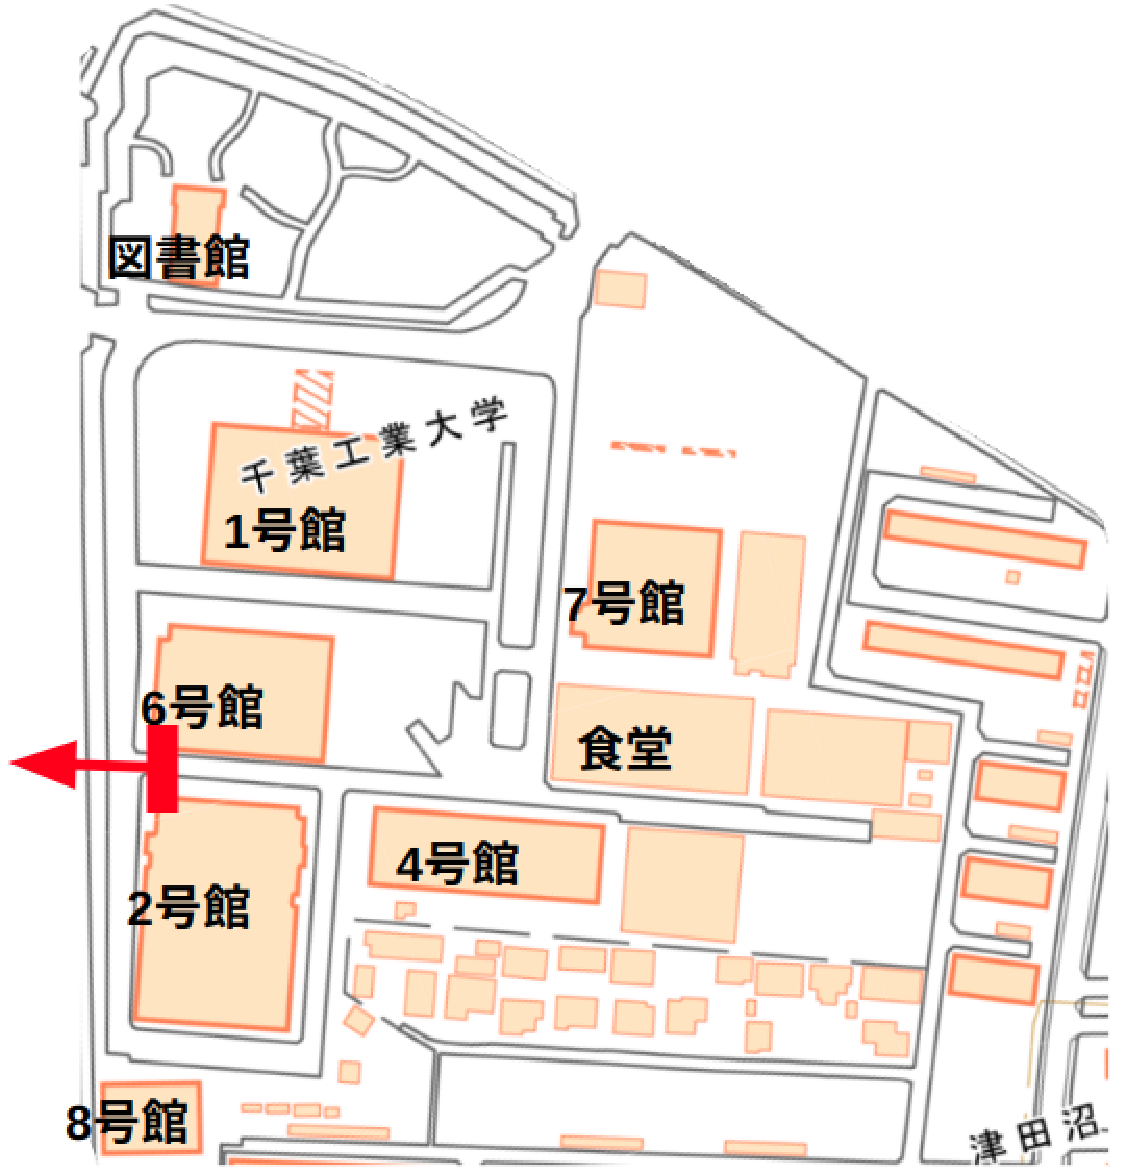
\includegraphics[keepaspectratio, scale=0.5]{images/png/ex_map3.pdf}
  \caption{Experiment location(source:\cite{mura})}
  \label{Fig:4.3}
\end{figure}

\begin{figure}[H]
  \centering
  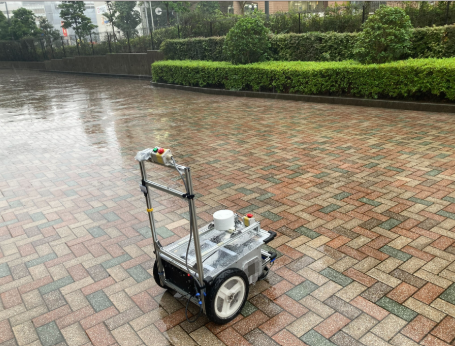
\includegraphics[keepaspectratio, scale=0.7]{images/png/ex.png}
  \caption{Experimental Setup}
  \label{Fig:4.4}
\end{figure}

\section{実験結果}
追加取得したデータ数を\tabref{table:Additional_number_of_data_acquired}に示す.
先行研究\cite{mura}と合わせたデータ数を\tabref{table:Total_number_of_data_acquired}に示す.
先行研究\cite{mura}同様に雨量が多いほど雨粒が頻繁に検出された.

\begin{table}[htbp]
  \centering
  \footnotesize
  \caption{The number of additional data points acquired under rainy weather conditions}
  \label{table:Additional_number_of_data_acquired}
  \begin{tabular}{|l|l|r|}
  \hline
  Rainfall & \multicolumn{1}{l|}{Number of data} \\
  \hline
  Range: 2.0 to 13 mm/h & 8 \\
  \hline
  \end{tabular}
\end{table}

\begin{table}[htbp]
  \centering
  \footnotesize
  \caption{The total number of data points acquired under rainy weather conditions.}
  \label{table:Total_number_of_data_acquired}
  \begin{tabular}{|l|l|r|}
  \hline
  Rainfall & \multicolumn{1}{l|}{Number of data} \\
  \hline
  Range: 2.0 to 13 mm/h & 30 \\
  \hline
  \end{tabular}
\end{table}